\section{Experiments}
\label{sec:experiment}

We evaluate \method on \bench across all seven domains, covering experimental setup (\S\ref{sec:exp:setup}), main evaluation results (\S\ref{sec:exp:main}), and cross-domain generalization (\S\ref{sec:exp:crossdomain}).
We additionally report supplementary rule-based verification results in Appendix~\ref{sec:appendix:rulebased} that corroborate the main findings.
As previewed in Figure~\ref{fig:bench_results_bar}, \method-397B-A17B achieves the highest overall score.

\begin{figure*}[t]
    \centering
    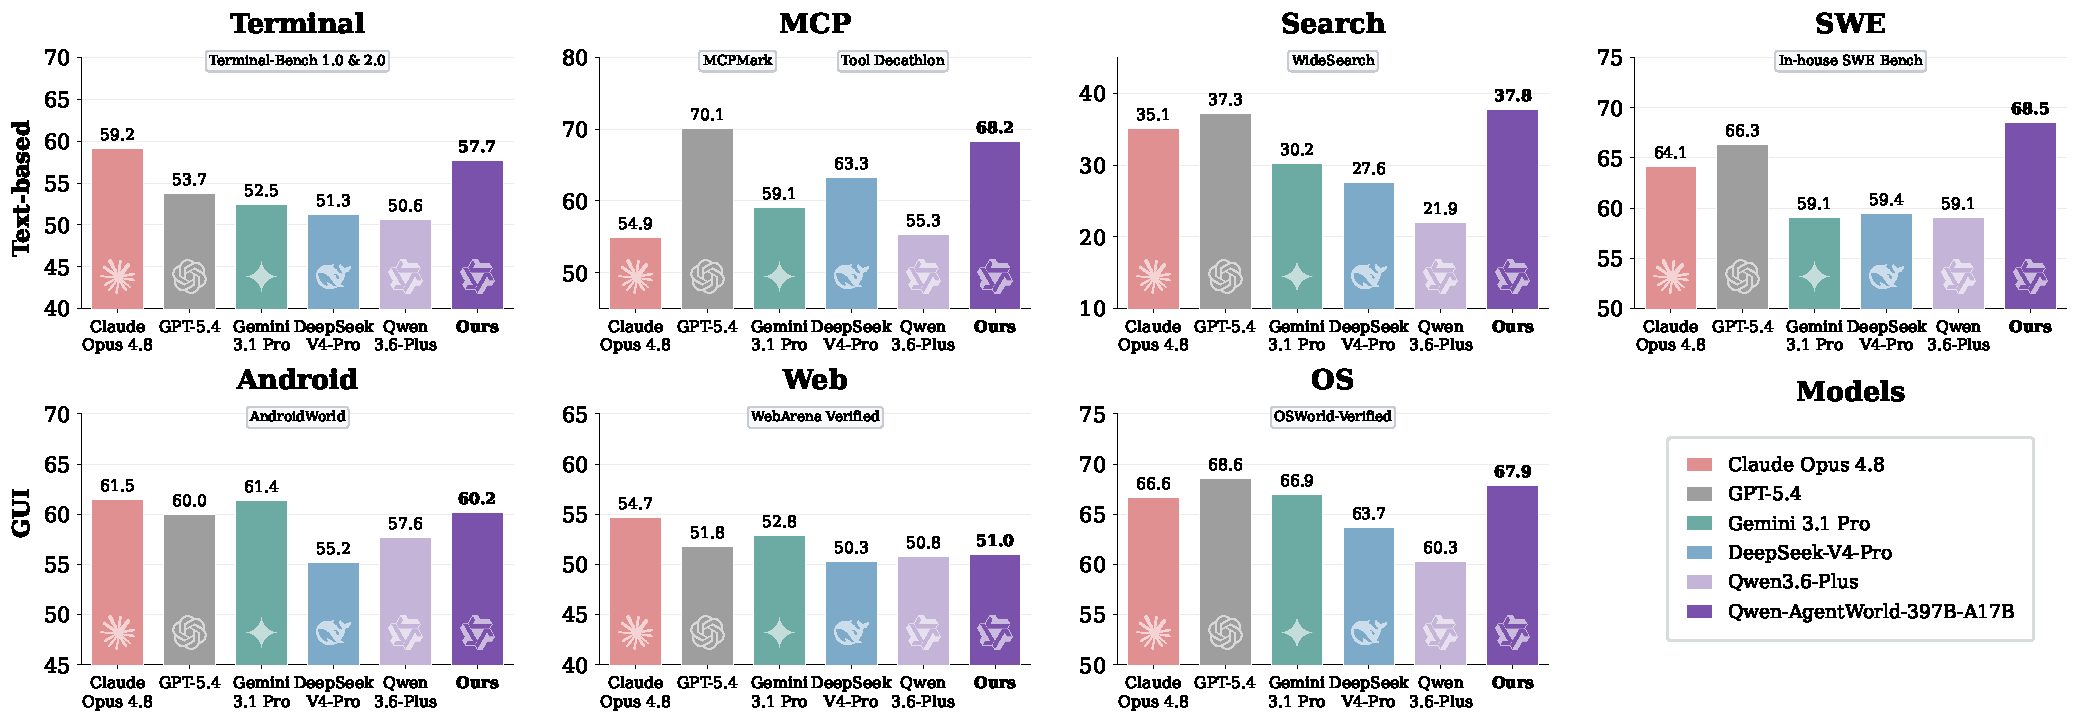
\includegraphics[width=\linewidth]{figures/bench_results_bar.pdf}
    \caption{Main results on \bench: five-dimensional rubric mean per domain. \method-397B-A17B achieves the highest overall average among all evaluated models, with consistent advantages on text-based domains and competitive performance on GUI domains.}
    \label{fig:bench_results_bar}
    \vspace{-4mm}
\end{figure*}

\subsection{Setup}
\label{sec:exp:setup}

\paragraph{Models.}
We evaluate \method-35B-A3B and \method-397B-A17B, both trained with the three-stage recipe of \S\ref{sec:pipeline}.

\paragraph{Baselines.}
We compare against 14 baselines spanning frontier proprietary models, open-weight models, and Qwen-family models without world-model training:
\begin{itemize}[nosep,leftmargin=*]
  \item \textit{Frontier Proprietary}: Claude Opus~4.8~\citep{opus4.8}, Claude Opus~4.6~\citep{opus4.6}, Claude Sonnet~4.6~\citep{sonnet4.6}, GPT-5.4~\citep{gpt-5.4}, Gemini~3.1~Pro~\citep{gemini3.1pro}.
  \item \textit{Open-Weight}: DeepSeek-V4-Pro~\citep{deepseekai2026deepseekv4}, Kimi~K2.6~\citep{team2026kimi}, GLM-5.1~\citep{zeng2026glm}, MiniMax-M2.7~\citep{minimax2026minimax}.
  \item \textit{Qwen Family (no LWM training)}: Qwen3.5-35B-A3B, Qwen3.5-397B-A17B~\citep{qwen35blog}, Qwen3.6-35B-A3B~\citep{qwen36_35b_a3b}, Qwen3.6-Plus~\citep{qwen36plus}, Qwen3.6-Max-Preview~\citep{qwen36_max_preview}.
\end{itemize}
The Qwen baselines isolate the effect of world-model training: they share the same base architecture but lack the three-stage CPT$\to$SFT$\to$RL pipeline.
In the result tables, the Qwen3.5 base checkpoints are placed alongside \method for direct comparison of the training effect.

\paragraph{Settings.}
All models use temperature~$=$~0.6 with thinking mode enabled where supported.
The maximum generation length and context length are set to the limits supported by each model.
Proprietary models use official API endpoints.
Open-weight models are deployed with SGLang.





\begin{table*}[t]
\caption{\bench main results: five-dimensional rubric mean ($\uparrow$) per domain. The highest and second-best scores per domain are shown in \textbf{bold} and \underline{underlined}, respectively.}
\label{tab:main_results}
\centering
\small
\setlength{\tabcolsep}{3.8pt}
\resizebox{.89\linewidth}{!}{%
\begin{tabular}{@{}ll cccc ccc c@{}}
\toprule
& \multirow{2}{*}{\textbf{Model}} & \multicolumn{4}{c}{\textbf{Text}} & \multicolumn{3}{c}{\textbf{GUI}} & \multirow{2}{*}{\textbf{Avg.}} \\
\cmidrule(lr){3-6} \cmidrule(lr){7-9}
& & \textbf{MCP} & \textbf{Search} & \textbf{Term.} & \textbf{SWE} & \textbf{Android} & \textbf{Web} & \textbf{OS} & \\
\midrule
\multirow{5}{*}{\rotatebox{90}{\scriptsize\textit{Frontier}}}
& Claude Opus~4.8          & 54.93 & 35.14 & \textbf{59.18} & 64.10 & \underline{61.50} & \textbf{54.66} & 66.62 & 56.59 \\
& Claude Opus~4.6          & 69.90 & 29.30 & 57.51 & 64.55 & \textbf{61.74} & 51.42 & \textbf{70.20} & 57.80 \\
& Claude Sonnet~4.6        & \underline{70.00} & 28.79 & 56.98 & 64.52 & 58.03 & 50.78 & 63.17 & 56.04 \\
& GPT-5.4                  & \textbf{70.10} & \underline{37.26} & 53.69 & \underline{66.29} & 60.00 & 51.80 & \underline{68.58} & \underline{58.25} \\
& Gemini~3.1~Pro           & 59.07 & 30.21 & 52.47 & 59.07 & 61.40 & \underline{52.83} & 66.92 & 54.57 \\
\midrule
\multirow{4}{*}{\rotatebox{90}{\scriptsize\textit{Open-weight}}}
& DeepSeek-V4-Pro          & 63.27 & 27.61 & 51.26 & 59.44 & 55.17 & 50.32 & 63.70 & 52.97 \\
& Kimi~K2.6                & 65.23 & 27.48 & 52.54 & 58.77 & 58.93 & 50.20 & 60.80 & 53.42 \\
& GLM-5.1                  & 67.60 & 22.46 & 47.32 & 52.07 & 59.10 & 51.50 & 59.13 & 51.31 \\
& MiniMax-M2.7             & 55.82 & 27.30 & 41.62 & 37.44 & 52.40 & 50.52 & 57.73 & 46.12 \\
\midrule
\multirow{3}{*}{\rotatebox{90}{\scriptsize\textit{Qwen}}}
& Qwen3.6-35B-A3B          & 42.96 & 18.78 & 43.81 & 40.71 & 51.88 & 46.53 & 55.48 & 42.88 \\
& Qwen3.6-Plus             & 55.28 & 21.94 & 50.58 & 59.08 & 57.65 & 50.78 & 60.33 & 50.81 \\
& Qwen3.6-Max-Preview      & 67.01 & 24.71 & 50.86 & 57.11 & 57.74 & 48.58 & 60.95 & 52.42 \\
\midrule
\multirow{4}{*}{\rotatebox{90}{\scriptsize\textit{Ours}}}
& Qwen3.5-35B-A3B          & 57.87 & 25.98 & 46.13 & 47.58 & 53.18 & 47.10 & 56.27 & 47.73 \\
& \method-35B-A3B          & 64.79 & 36.69 & 53.96 & 65.63 & 58.17 & 49.55 & 65.92 & 56.39 \\
\noalign{\vskip 2pt}
\cdashline{2-10}[6pt/3pt]
\noalign{\vskip 2pt}
& Qwen3.5-397B-A17B        & 68.31 & 30.81 & 55.30 & 64.44 & 54.90 & 48.55 & 60.85 & 54.74 \\
& \method-397B-A17B        & 68.24 & \textbf{37.82} & \underline{57.73} & \textbf{68.49} & 60.20 & 50.98 & 67.89 & \textbf{58.71} \\
\bottomrule
\end{tabular}%
}
\end{table*}

\subsection{Main Results}
\label{sec:exp:main}

Table~\ref{tab:main_results} reports the five-dimensional rubric mean across all seven domains.
Each predicted observation is scored on five rubric dimensions---\textit{Format}, \textit{Factuality}, \textit{Consistency}, \textit{Realism}, and \textit{Quality}---using a 1--5 scale, and then normalized to 0--100.
\method-397B-A17B achieves the highest overall average (58.71), surpassing GPT-5.4 (58.25) and all other frontier models.
On text-based domains, \method-397B-A17B leads with an average of 58.07, outperforming GPT-5.4 (56.84) by 1.23 points.
The advantage is most pronounced on Terminal (57.73 vs.\ 53.69) and SWE (68.49 vs.\ 66.29), the two domains where predictions require accurate modeling of code execution state and tool API behavior.
On GUI domains, Claude Opus~4.8 (60.93) and Claude Opus~4.6 (61.12) lead, followed by GPT-5.4 (60.47) and Gemini~3.1~Pro (60.04), with \method-397B-A17B ranking fifth (59.69).
The gap reflects an advantage from multimodal pre-training that text-only world modeling does not fully capture.

\paragraph{Effect of World-Model Training.}
Comparing \method with its base checkpoints isolates the contribution of the three-stage pipeline.
At the 397B scale, the overall average rises from 54.74 to 58.71.
At 35B, the gain is 8.66 points (47.73 to 56.39), lifting \method-35B-A3B above Claude Sonnet~4.6 (56.04) by 0.35 points.
The improvement is consistent across both text and GUI domains: at 397B, the text-domain average rises by 3.35 and the GUI-domain average by 4.92.
These gains are not explained by the base model's general capability alone, since the Qwen3.6 checkpoints without LWM training (Qwen3.6-Plus: 50.81, Qwen3.6-Max-Preview: 52.42) score well below \method despite sharing the same architecture family.

\paragraph{Domain-Level Observations.}
Search is the most challenging domain for all models: the best score (37.82) is roughly half the best score on SWE (68.49) or MCP (70.10).
Search requires modeling constantly evolving web content, and factual consistency across long retrieval chains remains difficult for all models.
On MCP, Claude Opus~4.6 and GPT-5.4 tightly at the top, reflecting their tool-use specialization.











\subsection{Cross-Domain Generalization}
\label{sec:exp:crossdomain}

\begin{figure*}[t]
    \centering
    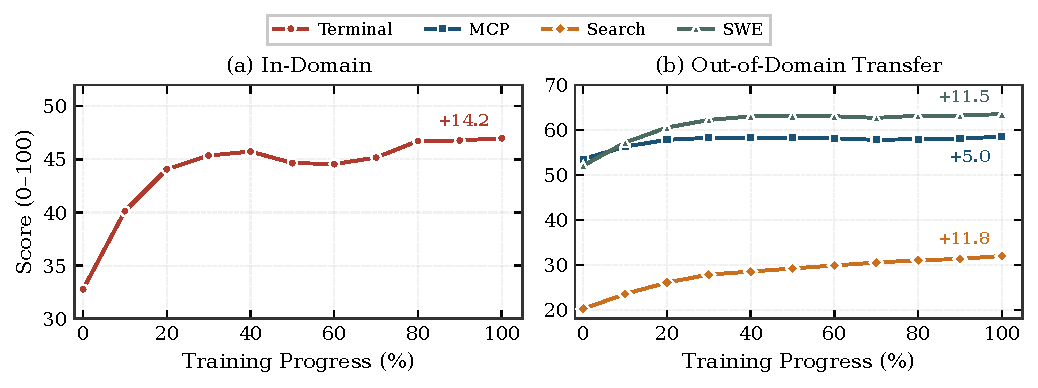
\includegraphics[width=\linewidth]{figures/cross_domain_transfer_v2.pdf}
    \caption{Cross-domain generalization when training Stage~3 (RL) on Terminal data alone. (a)~Terminal (in-domain) improves by +14.2 points over the SFT baseline. (b)~All three held-out domains improve without receiving any domain-specific training signal: MCP~(+5.0), SWE~(+11.5), and Search~(+11.8).}
    \label{fig:transfer_text}
    \vspace{-4mm}
\end{figure*}

This experiment tests whether \method learns generalizable language world knowledge or domain-specific environment behaviors.
We train Stage~3 (RL) on Terminal data alone and evaluate on all four text-based domains every 10 steps.
Figure~\ref{fig:transfer_text} shows the performance when training Stage~3 on Qwen3.5-35B-A3B-SFT, an in-house Qwen checkpoint that has undergone CPT and general-purpose SFT but no world-model training, using Terminal LWM data alone.
Terminal improves from 32.8 to 47.0 (+14.2) within 100 RL steps.
All three held-out text-based domains improve in parallel: SWE gains +11.5 (52.0 $\to$ 63.5), Search gains +11.8 (20.2 $\to$ 32.0), and MCP gains +5.0 (53.5 $\to$ 58.5) despite already starting from a high baseline.
The transfer is non-trivial: Terminal shell commands and MCP tool calls differ in syntax, state representation, and response structure, yet the gains emerge within the first 10 RL steps and remain stable throughout training.
This pattern suggests that RL reinforces generalizable world knowledge, how environments respond to actions, how errors propagate, how state transitions compose across turns, rather than domain-specific output formats.


